\section{Mathe Grundlagen}	

	\subsection{Partialbruchzerlegung}
		
\[f(x)=\frac{x^2+20x+149}{x^3+4x^2-11x-30} \Rightarrow \; \begin{array}{l}\text{Factorize denominator using}\\
	\text{Horner's scheme, binomial, etc.}\end{array} \Rightarrow
	x^{3}+4x^{2}-11x-30=(x+2)(x^{2}+2x-15)=(x+2)(x+5)(x-3)\] Approach:
	\[f(x)=\frac{x^2+20x+149}{x^3+4x^2-11x-30}=\frac{A}{x-3} + \frac{B}{x+2} + \frac{C}{x+5}=
	\frac{A(x+2)(x+5)+B(x-3)(x+5)+C(x-3)(x+2)}{(x-3)(x+2)(x+5)}\]
	Set up a system of equations with arbitrary values of $x_i$ (preferably choose poles or 0,1,-1):
	\[\begin{array}{l}x_1=3:\;-9+60+149=A\cdot5\cdot8\;\;\;\Rightarrow A=5\\
	x_2=-2:\;-4-40+149=B(-5)\cdot3\; \Rightarrow B=-7\\
	x_3=-5:\;-25-100+149=C(-8)(-3) \Rightarrow C=1 \end{array} \Rightarrow
	f(x)=\frac{5}{x-3}-\frac{7}{x+2}+\frac{1}{x+5}\] Additional approaches for other types of terms:
	\[f(x)=\frac{5x^2-37x+54}{x^3-6x^2+9x}=\frac{A}{x}+\frac{B}{x-3}+\frac{C}{(x-3)^2}=\frac{A(x-3)^2+Bx(x-3)+Cx}{x(x-3)^2}\]
	\[f(x)=\frac{1.5x}{x^3-6x^2+12x-8}=\frac{A}{x-2}+\frac{B}{(x-2)^2}+\frac{C}{(x-2)^3}=\frac{A(x-2)^2+B(x-2)+C}{(x-2)^3}\]
	\[f(x)=\frac{x^2-1}{x^3+2x^2-2x-12}=\frac{A}{x-2}+\frac{Bx+C}{x^2+4x+6}=\frac{A(x^2+4x+6)+(Bx+C)(x-2)}{(x-2)(x^2+4x+6)}\]

\subsubsection{Horner's Scheme}
	\begin{minipage}[t]{9cm}
		- Arrows $\Rightarrow$ Multiplication\\
		- Numbers in each column are added\\
		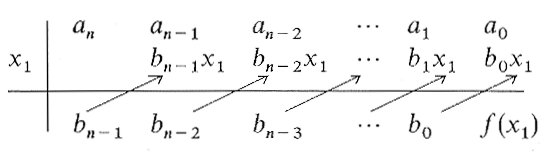
\includegraphics[width=6cm]{Content/04_calculation/hornerschema_1.png}\\
		$x_1 \Rightarrow$ Root (must be guessed!!)\\
		Top row = polynomial to be factored
	\end{minipage}
	\begin{minipage}[t]{9cm}
		\textbf{Example:}\\
		$f(x) = x^3-67x-126$\\
		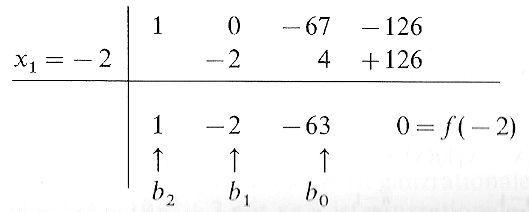
\includegraphics[width=6cm]{Content/04_calculation/hornerschema_2.png}\\
		$\Rightarrow f(x) = (x-x_1)(b_2x^2 + b_1x + b_0) = (x+2)(x^2-2x-63)$
	\end{minipage}

			
	\subsection{Trigonometrie}
			$\sin^2(b)+\cos^2(b)=1 \qquad \tan(b)=\frac{\sin(b)}{\cos(b)} \qquad \cosh(b)^2 - \sinh(b)^2 = 1 \qquad \tanh(b)=\frac{\sinh(b)}{\cosh(b)}$
\subsubsection{Funktionswerte für Winkelargumente}
	\renewcommand{\arraystretch}{1.5}
	\begin{minipage}{5cm}
		\begin{tabular}[c]{ |c|c||c|c|c| }
	    	\hline
			deg & rad & sin & cos & tan\\
			\hline
			0\symbol{23} & 0 & 0 & 1 & 0\\
			\hline
			30\symbol{23} & $\frac{\pi}{6}$ & $\frac{1}{2}$ & $\frac{\sqrt{3}}{2}$ &
			$\frac{\sqrt{3}}{3}$\\
			\hline
			45\symbol{23} & $\frac{\pi}{4}$ & $\frac{\sqrt{2}}{2}$ & $\frac{\sqrt{2}}{2}$
			& 1\\
			\hline
			60\symbol{23} & $\frac{\pi}{3}$ & $\frac{\sqrt{3}}{2}$ & $\frac{1}{2}$ &
			$\sqrt{3}$\\
			\hline			
		\end{tabular}			
	\end{minipage}
	\begin{minipage}{4.3cm}
		\begin{tabular}[c]{ |c|c||c|c|}
	    	\hline
			deg & rad & sin & cos\\
			\hline
			90\symbol{23} & $\frac{\pi}{2}$ & 1 & 0\\
			\hline	
			120\symbol{23} & $\frac{2\pi}{3}$ & $\frac{\sqrt{3}}{2}$ & $-\frac{1}{2}$ \\
			\hline
			135\symbol{23} & $\frac{3\pi}{4}$ & $\frac{\sqrt{2}}{2}$ & $-\frac{\sqrt{2}}{2}$\\
			\hline
			150\symbol{23} & $\frac{5\pi}{6}$ & $\frac{1}{2}$ & $-\frac{\sqrt{3}}{2}$\\
			\hline
		\end{tabular}			
	\end{minipage}
	\begin{minipage}{4.5cm}
		\begin{tabular}[c]{ |c|c||c|c| }
	    	\hline
			deg & rad & sin & cos\\
			\hline
			180\symbol{23} & $\pi$ & 0 & -1\\
			\hline	
			210\symbol{23} & $\frac{7\pi}{6}$ & $-\frac{1}{2}$ & $-\frac{\sqrt{3}}{2}$\\
			\hline
			225\symbol{23} & $\frac{5\pi}{4}$ & $-\frac{\sqrt{2}}{2}$ & $-\frac{\sqrt{2}}{2}$\\
			\hline
			240\symbol{23} & $\frac{4\pi}{3}$ & $-\frac{\sqrt{3}}{2}$ & $-\frac{1}{2}$\\
			\hline
		\end{tabular}			
	\end{minipage}
	\begin{minipage}{4.5cm}
		\begin{tabular}[c]{ |c|c||c|c| }
	    	\hline
			deg & rad & sin & cos\\
			\hline
			270\symbol{23} & $\frac{3\pi}{2}$ & -1 & 0\\
			\hline	
			300\symbol{23} & $\frac{5\pi}{3}$ & $-\frac{\sqrt{3}}{2}$ & $\frac{1}{2}$\\
			\hline
			315\symbol{23} & $\frac{7\pi}{4}$ & $-\frac{\sqrt{2}}{2}$ & $\frac{\sqrt{2}}{2}$\\
			\hline
			330\symbol{23} & $\frac{11\pi}{6}$ & $-\frac{1}{2}$ & $\frac{\sqrt{3}}{2}$\\
			\hline
		\end{tabular}			
	\end{minipage}
	\renewcommand{\arraystretch}{1}
	
\subsubsection{Quadrantenbeziehungen}
	\begin{tabbing}
    	xxxxxxxxxxxxxxxxxxxxxxxxxxxxxxxxxx \= \kill
	  	$\sin(-a)=-\sin(a)$ \> $\cos(-a)=\cos(a)$\\
		$\sin(\pi - a)=\sin(a)$ \> $\cos(\pi - a)=-\cos(a)$\\
		$\sin(\pi + a)=-\sin(a)$ \> $\cos(\pi +a)=-\cos(a)$\\
		$\sin\left(\frac{\pi}{2}-a \right)=\sin\left(\frac{\pi}{2}+a \right)=\cos(a)$ \>
		$\cos\left(\frac{\pi}{2}-a \right)=-\cos\left(\frac{\pi}{2}+a \right)=\sin(a)$  
    \end{tabbing}

	\textbf{Additionstheoreme}
		$\sin(a \pm b)=\sin(a) \cdot \cos(b) \pm \cos(a) \cdot \sin(b) \qquad
		\cos(a \pm b)=\cos(a) \cdot \cos(b) \mp \sin(a) \cdot \sin(b)$\\ 
		$\tan(a \pm b)=\dfrac{\tan(a) \pm \tan(b)}{1 \mp \tan(a) \cdot \tan(b)}$
		
	\subsubsection{Doppel- und Halbwinkel}	
		\begin{tabular}{ll}
			$\sin(2a)=2\sin(a)\cos(a)$ &
			$\cos(2a)=\cos^2(a)-\sin^2(a)=2\cos^2(a)-1=1-2\sin^2(a)$\\
			$\cos^2 \left(\frac{a}{2}\right)=\frac{1+\cos(a)}{2}$ &
			$\sin^2 \left(\dfrac{a}{2}\right)=\frac{1-\cos(a)}{2}$
		\end{tabular}\\
		
	\begin{minipage}[t]{9.5cm}	
		\subsubsection{Produkte}
			$\sin(a)\sin(b)=\frac{1}{2}(\cos(a-b)-\cos(a+b))$\\
			$\cos(a)\cos(b)=\frac{1}{2}(\cos(a-b)+\cos(a+b))$\\
			$\sin(a)\cos(b)=\frac{1}{2}(\sin(a-b)+\sin(a+b))$
		\subsubsection{Hyperbolic}
			$\sinh(z) = \frac{1}{2} \left( e^z - e^{-z} \right) \qquad \cosh(z) =
			\frac{1}{2} \left( e^z + e^{-z} \right) $
	\end{minipage}
	\hfill
	\begin{minipage}[t]{9.5cm}		
		\subsubsection{Summe und Differenz}
			$\sin(a)+\sin(b)=2 \cdot \sin \left(\frac{a+b}{2}\right) \cdot
			\cos\left(\frac{a-b}{2}\right)$\\
			$\sin(a)-\sin(b)=2 \cdot \sin \left(\frac{a-b}{2}\right) \cdot
			\cos\left(\frac{a+b}{2}\right)$\\
			$\cos(a)+\cos(b)=2 \cdot \cos \left(\frac{a+b}{2}\right) \cdot
			\cos\left(\frac{a-b}{2}\right)$\\
			$\cos(a)-\cos(b)=-2 \cdot \sin \left(\frac{a+b}{2}\right) \cdot
			\sin\left(\frac{a-b}{2}\right)$\\
			$\tan(a) \pm \tan(b)=\dfrac{\sin(a \pm b)}{\cos(a)\cos(b)}$
	\end{minipage}	
	
		
	\subsubsection{Euler}
	$sin(z)=\frac{e^{jz}-e^{-jz}}{2j} \hspace{2cm}
    cos(z)=\frac{e^{jz}+e^{-jz}}{2} \hspace{2cm}
    e^{j\varphi}=cjs(\varphi)=cos(\varphi)+j sin(\varphi)$
    
    \subsubsection{Komplex}
    \begin{tabular}{lll}
     	Betrag: & $ |z| = \sqrt{Re(z)^2 + Im(z)^2} = \sqrt{z \cdot \bar{z}}$\\ 
     	Konjugiertkomplex: & $z=z_1 + jz_2$ & $\bar{z}=z^*=z_1-jz_2$
     \end{tabular}
	
			
	\subsection{Taylor Polynom}
		$f(x_0+h)=f(x_0) + f'(x_0)h + \frac{f''(x_0)}{2}h^2 + \frac{f'''(x_0)}{3!}h^3 + \ldots + \frac{f^{(n)}(x_0)}{n!}h^n + R_n(x_0, h)$

	\subsection{Integralrechnung}	
	\begin{tabbing}
	     xxxxxxxxxxxxxxxxxxxxxxxxxxxxxxx \= xxx \= xxxxxxxxxxxxxxxxxxxxxxxxxxxxxxxxxxxxxxxxxxxxxxxxxxxxxxx\kill  
	     Integration\>\>$A=\int\limits_{a}^{b}{f(t)dt}=\left[F(t)\right]_a^b=F(b)-F(a)$\\[0.2cm]
	     Linearität\>		  
	   $\qquad\int{f(\alpha x+\beta )dx=\frac{1}{\alpha}\cdot F(\alpha x+
				\beta)+C}$\\[0.2cm]
		   Partielle Integration\>
	   $\qquad\int\limits_a^b{\underset{\Uparrow}{u}'(x)\cdot \underset{\Downarrow}{v}(x)dx}=\biggl[ u(x)\cdot v(x) \biggr]_a^b
	   -\int\limits_a^b{u(x)\cdot v'(x)dx}$\\[0.2cm]
	   Substitution (Rationalisierung)\>
	   $\qquad t=\tan\frac{x}{2}, \qquad dx=\frac{2dt}{1+t^2} \qquad 
	   \sin  x=\frac{2t}{1+t^2} \qquad \cos x=\frac{1-t^2}{1+t^2}
				\quad\int{R(\sin(x)\cos(x))dx}$\\ 
	   Allgemeine Substitution \> \>
				$\int\limits_{a}^{b}{f(x)dx}=\int\limits_{g^{-1}(a)}^{g^{-1}(b)}{f(g(t))\cdot
				g'(t)dt}\qquad t=g^{-1}(x)\qquad  \fbox{x=g(t)}\qquad dx=g'(t)\cdot dt$\\
	   Logarithmische Integration \>\>
	    $ \int{\frac{f'(x)}{f(x)}dx}=\ln|f(x)|+C	\qquad{(f(x)\neq 1)}$\\[0.2cm]
	  Spezielle Form des Integranden \>\>
		 		$\int{f'(x)\cdot (f(x))^{\alpha} dx}= f(x)^{\alpha +1}\cdot
		 		\frac{1}{\alpha+1}+C \qquad{(\alpha \neq -1)}$\\ 
	   Differentiation\>\>
		 		$\int \limits ^{b} _{a} {f'(t)dt}=f(b)-f(a)$\qquad
				$\frac{d}{dx} \int \limits ^{x} _{1} {f(t)dt}=f(x)$
	\end{tabbing}
	%\subsubsection{Einige unbestimmte Integrale}
	%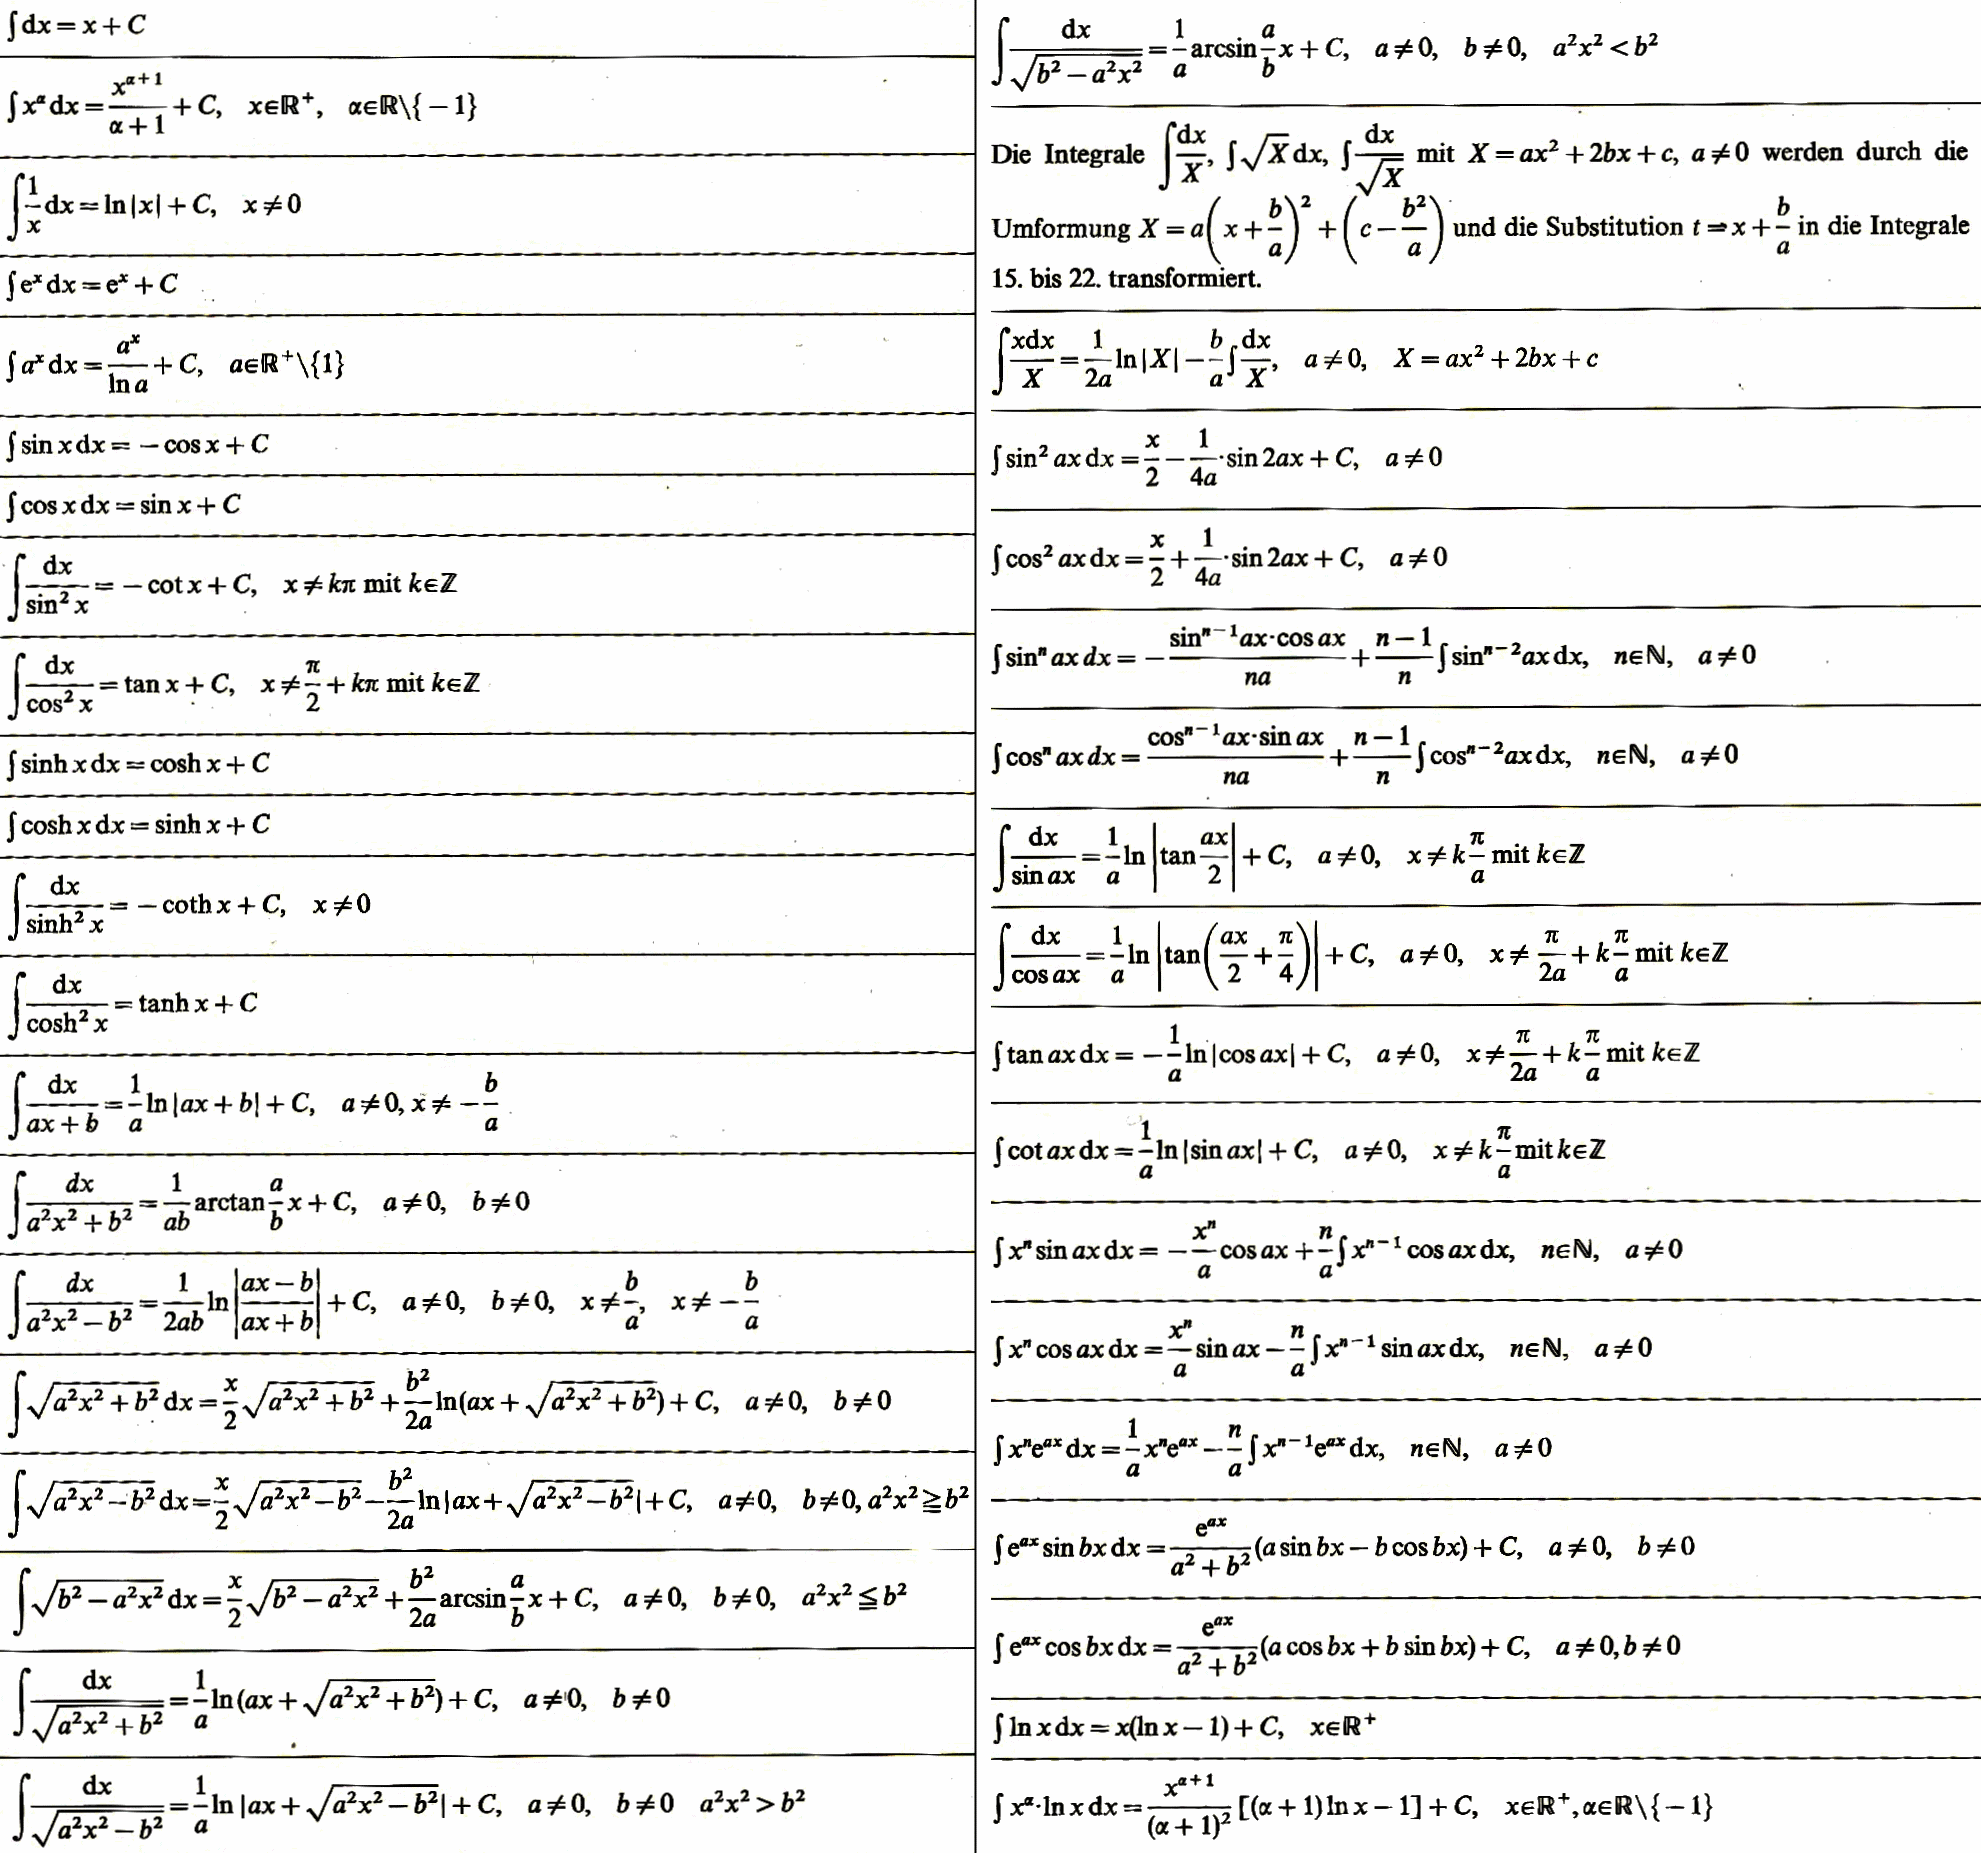
\includegraphics[width=19cm]{Content/Rechenregeln/integrale.png} 
	
	$\int \mathrm dx = x + C$\\
	$\int x^{\alpha} \mathrm dx = \frac{x^{\alpha + 1}}{\alpha + 1} + C$, $x \in
	\mathbb{R}^+$, $\alpha \in \mathbb{R} \textbackslash \{-1\}$\\
	$\int \frac{1}{x} \mathrm dx = \ln \lvert x \lvert + C$, $x \neq 0$\\
	$\int e^x \mathrm dx = e^x + C$\\
	$\int a^x \mathrm dx = \frac{a^x}{\ln(a)} + C$, $a \in \mathbb{R}^+
	\textbackslash \{1\}$\\
	$\int \sin x \mathrm dx = - \cos x + C$\\
	$\int \cos x \mathrm dx = \sin x + C$\\
	$\int \frac{\mathrm dx}{\sin^2 x} = -\cot(x) + C$, $x \neq k \pi$ mit $k \in
	\mathbb{Z}$\\
	$\int \frac{\mathrm dx}{\cos^2 x} = \tan(x) + C$, $x \neq \frac{\pi}{2} + k \pi$
	mit $k \in \mathbb{Z}$\\
	$\int \sinh(x) \mathrm dx = \cosh(x) + C$\\
	$\int \cosh(x) \mathrm dx = \sinh(x) + C$\\
	$\int \frac{\mathrm dx}{\sinh^2 x} = -\coth(x) + C$, $x \neq 0$\\
	$\int \frac{\mathrm dx}{\cosh^2 x} = \tanh(x) + C$, $x \neq 0$\\
	$\int \frac{\mathrm dx}{ax + b} = \frac{1}{a} \ln \lvert ax + b \lvert + C$, $a
	\neq 0$, $x \neq - \frac{b}{a}$\\
	$\int \frac{\mathrm dx}{a^2x^2 + b^2} = \frac{1}{ab} \arctan(\frac{a}{b} x) +
	C$, $a \neq 0$, $x \neq - \frac{b}{a}$ $x \neq -\frac{b}{a}$\\
	$\int \frac{\mathrm dx}{a^2x^2 - b^2} = \frac{1}{2ab} \ln \lvert \frac{ax -
	b}{ax + b} \lvert + C$, $a \neq 0$, $x \neq - \frac{b}{a}$ $x \neq
	-\frac{b}{a}$\\
	$\int \sqrt{a^2 x^2 + b^2} \mathrm dx = \frac{x}{2} \sqrt{a^2 x^2 + b^2} +
	\frac{b^2}{2a} \ln(ax + \sqrt{a^2 x^2 + b^2}) + C$, $a \neq 0$, $b \neq 0$\\
	$\int \sqrt{a^2 x^2 - b^2} \mathrm dx = \frac{x}{2} \sqrt{a^2 x^2 - b^2} +
	\frac{b^2}{2a} \ln \lvert ax + \sqrt{a^2 x^2 - b^2} \lvert + C$, $a \neq 0$, $b
	\neq 0$, $a^2 x^2 \geq b^2$\\
	$\int \sqrt{b^2 - a^2x^2} \mathrm dx = \frac{x}{2} \sqrt{b^2 - a^2x^2} +
	\frac{b^2}{2a} \arcsin(\frac{a}{b} x) + C)$, $a \neq 0$, $b \neq 0$,
	$a^2 x^2 \geq b^2$\\
	$\int \frac{\mathrm dx}{\sqrt{a^2 x^2 + b^2}} = \frac{1}{a} \ln(ax +
	\sqrt{a^2 x^2 + b^2}) + C$, $a \neq 0$, $b \neq 0$\\
	$\int \frac{\mathrm dx}{\sqrt{a^2 x^2 - b^2}} = \frac{1}{a} \ln(ax +
	\sqrt{a^2 x^2 - b^2}) + C$, $a \neq 0$, $b \neq 0$ $a^2 x^2 > b^2$\\
	$\int \frac{\mathrm dx}{\sqrt{b^2 - a^2 x^2}} = \frac{1}{a}
	\arcsin(\frac{a}{b} x) + C$, $a \neq 0$, $b \neq 0$, $a^2 x^2 < b^2$\\
	Die Integrale $\int \frac{dx}{X}$, $\int \sqrt{X} \; dx$, $\int
	\frac{dx}{\sqrt{X}}$ mit $X = ax^2 + 2bx + c$, $a \neq 0$, werden durch die
	Umformung $X = a \left(x + \frac{b}{a}\right)^2 + \left(c -
	\frac{b^2}{a}\right)$ und die Substitution $t = x + \frac{b}{a}$ in die
	Integrale 15. bis 22. transformiert.\\
	$\int \frac{x \; \mathrm dx}{X}= \frac{1}{2a} \ln \lvert X \lvert - \frac{b}{a}
	\int \frac{dx}{X}$, $a \neq 0$, $X = ax^2 + 2bx + c$\\
	$\int \sin^2(ax) \; \mathrm dx = \frac{x}{2} - \frac{1}{4a} \cdot \sin(2ax) +
	C$, $a \neq 0$\\
	$\int \cos^2(ax) \; \mathrm dx = \frac{x}{2} + \frac{1}{4a} \cdot \sin(2ax) +
	C$, $a \neq 0$\\
	$\int \sin^n(ax) \; \mathrm dx = \frac{\sin^{n-1}(ax) \cdot \cos(ax)}{na} +
	\frac{n-1}{n} \int \sin^{n-2}(ax) \mathrm dx$, $n \in \mathbb N$, $a \neq 0$\\
	$\int \cos^n(ax) \; \mathrm dx = \frac{cos^{n-1}(ax) \cdot \sin(ax)}{na} +
	\frac{n-1}{n} \int \cos^{n-2}(ax) \mathrm dx$, $n \in \mathbb N$, $a \neq 0$\\
	$\int \frac{dx}{\sin (ax)} = \frac{1}{a} \ln \lvert \tan(\frac{ax}{2}) \lvert +
	C$, $a \neq 0$, $x \neq k \frac{\pi}{a}$ mit $k \in \mathbb Z$\\
	$\int \frac{dx}{cos (ax)} = \frac{1}{a} \ln \lvert \tan(\frac{ax}{2} +
	\frac{\pi}{4}) \lvert + C$, $a \neq 0$, $x \neq \frac{\pi}{2a} + k
	\frac{\pi}{a}$ mit $k \in \mathbb Z$\\
	$\int \tan(ax) \mathrm dx = - \frac{1}{a} \ln \lvert \cos(ax) \lvert + C$, $a
	\neq 0$, $x \neq \frac{\pi}{2a} + k \frac{\pi}{a}$ mit $k \in \mathbb Z$\\
	$\int \cot(ax) \mathrm dx = \frac{1}{a} \ln \lvert \sin(ax) \lvert + C$, $a
	\neq 0$, $x \neq k \frac{\pi}{a}$ mit $k \in \mathbb Z$\\
	$\int x^n \sin(ax) \mathrm dx = - \frac{x^n}{a} \cos(ax) + \frac{n}{a} \int
	x^{n-1} \cos(ax) \mathrm dx$, $n \in \mathbb N$, $a \neq 0$\\
	$\int x^n \cos(ax) \mathrm dx = \frac{x^n}{a} \sin(ax) - \frac{n}{a} \int
	x^{n-1} \sin(ax) \mathrm dx$, $n \in \mathbb N$, $a \neq 0$\\
	$\int x^n e^{ax} \mathrm dx = \frac{1}{a} x^n e^{ax} - \frac{n}{a} \int
	x^{n-1} e^{ax} \mathrm dx$, $n \in \mathbb N$, $a \neq 0$\\
	$\int e^{ax} \sin(bx) \mathrm dx = \frac{e^{ax}}{a^2 + b^2} (a \cdot \sin(bx) -
	b \cdot \cos(bx)) + C$, $a \neq 0$, $b \neq 0$ \\
	$\int e^{ax} \cos(bx) \mathrm dx = \frac{e^{ax}}{a^2 + b^2} (a \cdot \cos(bx) +
	b \cdot \sin(bx)) + C$, $a \neq 0$, $b \neq 0$ \\
	$\int \ln(x) \mathrm dx = x(\ln(x) - 1) + C$, $x \in \mathbb R^+$\\
	$\int x^\alpha \cdot \ln(x) \mathrm dx = \frac{x^{\alpha + 1}}{(\alpha + 1)^2}
	[(\alpha + 1) \ln(x) - 1] + C$, $x \in \mathbb R^+$, $\alpha \in \mathbb R
	\textbackslash \{-1\}$\\
	
			
	\subsection{Differentialgleichungen}
		
	\subsubsection{Linear Differential Equation of 1. Order}
	\begin{tabular}{lll}
	\textbf{Form:} $ y'+f(x)y = g(x) $ &
	\textbf{Procedure:} $y=y_H+y_p$ &
	$y_H=k \cdot e^{-\int f(x) dx}$ where $k=y_0$\\ & &
	$y_p=k \cdot e^{-\int f(x) dx}$ where $k=\int(g(x) \cdot e^{\int f(x) dx}) dx$
	\end{tabular}

	\subsubsection{Linear Differential Equation 2nd Order with Constant Coefficients}
	\begin{tabular}{p{8cm}p{8cm}}
	\textbf{Form:} $y''+a_1\cdot y'+a_0\cdot y=f(x)$  &
	\textbf{Forcing Term:} $f(x)$\\
	\textbf{Homogeneous Differential Equation:} $f(x)=0$ &
	\textbf{Inhomogeneous Differential Equation:} $f(x)\neq 0$
	\end{tabular}

	\subsubsection{General Solution of a Homogeneous ODE:\quad\subsubadd{$\quad
	Y_H$}}
	\textbf{Characteristic Polynomial}
	$\qquad\underline{\lambda^2+a_1\cdot\lambda+a_0=0}$ \hspace{1cm}of
	$\qquad\underline{y''+a_1\cdot y'+a_0\cdot y=0}$
	$\qquad(\lambda_{1,2} = -\frac{a_1}{2} \pm \frac{\sqrt{a_1^2 - 4a_0}}{2})$\\ \\
	\begin{tabular}{p{8cm}p{8cm}}
	If $\lambda_1\neq \lambda_2$ and $\lambda_{1,2} \in R$:&
	$Y_H=Ae^{\lambda_1x}+Be^{\lambda_2x}$\\
	If $\lambda_1=\lambda_2$ and $\lambda_{1,2} \in R$:    &
	$Y_H=e^{\lambda_1x}(A+B\cdot x)$\\
	If $\lambda_{1,2}=-\frac{a_1}{2}\pm j\alpha$:          &
	$Y_H=e^{-\frac{1}{2}a_1x}(A\cos(\alpha x) +B\sin(\alpha x))$\\
	\end{tabular}\\

	\subsubsection{General Solution of an Inhomogeneous ODE:\quad\subsubadd{$y=Y_H+y_P$}}

	\textbf{Basic Solution Method of an Inhomogeneous ODE:\quad\subsubadd{$\quad y_P$}}\\
	Homogeneous ODE: $y''+a_1\cdot y'+a_0\cdot y=0$  for which ($g(x)=Y_H$ homogeneous solution)  $g(x_0)=0$  and
	$g'(x_0)=1$  holds, is:\\
	$$y_P(x)=\int\limits_{x_o}^{x} g(x+x_0-t)\cdot f(t)dt$$\\
	the particular solution of $y''+a_1\cdot y'+a_0\cdot y=f(x)$\\

	\textbf{The Approach of an Inhomogeneous ODE in the Form of
	The Forcing Term:\quad\subsubadd{$\quad y_P$}}\\

	 $f(x)=p_n(x)$\hspace{9cm}($p_n(x)$
	and $q_n(x)$ are polynomials of the same degree)\\
	\begin{tabular}{p{8cm}p{4cm}}
	Case a: $a_0\neq 0$:          & $y_P = q_n(x)$\\
	Case b: $a_0 = 0 , a_1\neq 0$:& $y_P=x\cdot q_n(x)$\\
	Case c: $a_0=a_1=0$:          & $y_P=x^2\cdot q_n(x)$\\
	\end{tabular}\\
	\\

	$f(x)=e^{bx}\cdot p_n(x)$\\
	\begin{tabular}{p{8cm}p{4cm}}
	Case a: $b$ not a root of the characteristic polynomial:    &
	$y_P=e^{bx}\cdot q_n(x)$\\
	Case b: $b$ a simple root of the characteristic polynomial: &
	$y_P=e^{bx}\cdot x \cdot q_n(x)$\\
	Case c: $b$ a double root of the characteristic polynomial:&
	$y_P=e^{bx}\cdot x^2\cdot q_n(x)$\\
	\end{tabular}\\
	\\

	$f(x)=e^{cx}\cdot (p_n(x)\cos(bx)+q_n(x)\sin(bx))$\\
	\begin{tabular}{p{8cm}p{8cm}}
	Case a: $c+jb$ not a solution of the characteristic equation:    &
	$y_P=e^{cx}\cdot (r_n(x)\cos(bx)+s_n(x)\sin(bx))$\\
	Case b: $c+jb$ a solution of the characteristic equation: &
	$y_P=e^{cx}\cdot x\cdot(r_n(x)\cos(bx)+s_n(x)\sin(bx))$\\
	\end{tabular}\\
	\\

	\textbf{Superposition Principle}

	$f(x)=c_1f_1(x)+c_2f_2(x)$\\
	\begin{tabular}{p{8cm}p{4cm}}
	$y_1$ is a specific solution of the ODE &
	$y''+a_1\cdot y'+a_0\cdot y=c_1f_1(x)$ \\
	$y_2$ is a specific solution of the ODE &
	$y''+a_1\cdot y'+a_0\cdot y=c_2f_2(x)$ \\
	then:                          &
	$y_P=c_1y_1+c_2y_2$\\
	\end{tabular}


	\newpage

	\subsubsection{Linear Differential Equation of nth Order with Constant Coefficients}
	\begin{tabular}{p{4cm}p{12cm}}
	\textbf{Form:} &
	$y^{(n)}+a_{n-1}\cdot y^{(n-1)}+\ldots +a_0\cdot y=f(x)$ $\Leftrightarrow$ $\sum\limits_{k=0}^na_ky^{(k)}=f(x)$\\
	\end{tabular}

	\textbf{Homogeneous Solutions}\\
	\begin{tabular}{lll}
	Case a: r real solutions $\lambda$:
		& $y_1=e^{\lambda x}$, $y_2=xe^{\lambda x}$, \ldots
		,$y_r=x^{r-1}e^{\lambda x}$
		& Strong damping/creeper case\\
	Case b: $k$ complex solutions $\lambda=\alpha +j\beta$:
		&$y_1=e^{\alpha x}\cos(\beta x)$, $y_{3}=e^{\alpha x}x^1\cos(\beta
	x),...$ (odd)
		& Weak damping /\\
		&$y_{2}=e^{\alpha x}\sin(\beta x)$, $y_{4}=e^{\alpha
	x}x^{1}\sin(\beta x),...$ (even)
		& Oscillation case\\
	\end{tabular}

	Degrees of freedom $(A,B,C, ...)$ and additional $x^{n}$ should not be forgotten!!!

	\textbf{Most General Solution of the Particular Part:}\\
	$$\underbrace{\sum_{k=0}^n a_k y^{(k)}}_{f(y,y',y'',\ldots)} = \underbrace{e^{\alpha x} (p_{m1}(x) \cos (\beta x) + q_{m2}(x) \sin (\beta x))}_{\text{Forcing term}}$$
	Distinguish solutions of the characteristic polynomial ($\lambda$):\hspace{5.5cm}with m = max(m1, m2)\\
	\begin{tabular}{p{8cm}p{8.5cm}}
	Case a: $\alpha + j\beta \neq \lambda$, then &
	$y_P = e^{\alpha x}(r_m(x)\cos(\beta x) + s_m(x) \sin(\beta x))$\\
	Case b: $\alpha + j\beta$  is a u-fold solution of $\lambda$, then &
	$y_P = e^{\alpha x} x^u (r_m(x) \cos(\beta x) + s_m(x) \sin(\beta x))$\\
	&
	u-fold resonance

	\end{tabular}

	\textbf{Basic Solution Method}\\
	\begin{tabular}{p{12cm}p{5cm}}
	$\begin{pmatrix}
	g(x_0)=  & 0 & = & c_1g_1(x_0)+c_2g_2(x_0)+\ldots +c_n(x_0)\\
	g'(x_0)= & 0 & = & c_1g_1'(x_0)+c_2g_2'(x_0)+\ldots +c_ng_n'(x_0)\\
	\vdots  & \vdots & \\
	g^{(n-1)}(x_0)= & 1 & = & c_1g_1^{(n-1)}(x_0)+c_2g_2^{(n-1)}(x_0)+\ldots
	+c_ng_n^{(n-1)}(x_0)
	\end{pmatrix}$ &
	\begin{minipage}[t]{5cm}
	Results in $c_1,\ldots ,c_n$ for\\
	$y_{P}(x)=\int_{x_0}^x{g(x+x_0-t)f(t)dt}$
	\end{minipage}
	\end{tabular}


	\subsubsection{Linear Differential Equation Systems of First Order with Constant Coefficients}
	\begin{tabular}{p{8cm}p{8cm}}
	\textbf{Form:}&
	$\dot{x}=ax+by+f(t) \leftrightarrow y=\frac{1}{b}(\dot{x}-ax-f(t))$\\
	&
	$\dot{y}=cx+dy+g(t)$\\
	\textbf{The general solution results from the ODE:}&
	$\ddot{x}-(a+d)\dot{x}+(ad-bc)x=\dot{f}(t)-d \cdot f(t)+b \cdot g(t)$\\
	\end{tabular}

	$\ddot{x}, \dot{x}, \dot{y}$ are each differentiated with respect to $t$!

	\subsubsection{Solving ODEs with Laplace Transformation}
		To solve an ODE with Laplace (causal!), the equation must first be transformed into the Laplace domain.
		After that, the equation can be solved algebraically.
		The result must then be transformed back into the original domain through inverse transformation.  \\

		Note:\\
		- $H(s)=\frac{1}{p(s)}$ where $p(s)$ represents the characteristic polynomial

		\textbf{Stability}\\
			A system is stable if the root of the characteristic polynomial $p(s)$ lies in the left half-plane:\\
			$$Re[p(s)] < 0$$


	\subsubsection{Common DEs}
	  \label{sec:dgls}
	  \begin{tabular}{ll | ll}
	    DE & Solution & DE & Solution\\[0.2cm]
        $\dfrac{dx}{dt} =0$
        & $C$
 	    & $\dfrac{dx}{dt} =1$
 	    & $t + C$\\[0.2cm]
	    $\dfrac{dx}{dt} = y$
	    & $t \cdot y + C$
	    & $\dfrac{dx}{dt} = kx$
	    & $C e^{kt}$\\[0.2cm]
	    $\dfrac{d u}{dt} = \sin(t)$
	    & $C - \cos(t)$
	    & $\dfrac{d^2 x}{dt^2} = k^2x$
	    & $A*\cosh(kt) + B*\sinh(kt) = \dfrac{1}{2}((A+B)e^{kt} + (A-B)e^{-kt})$\\[0.2cm]
	    $\dfrac{d^2 x(t)}{dt^2} = -\omega^2 x(t)$
	    & $A \cos(\omega t) + B \sin(\omega t)$
	    & &
	  \end{tabular}

	\subsection{Differential-Rechnung}
	  $f'(x_0)=\lim\limits_{\Delta x\rightarrow 0}
	  \frac{f(x_0+\Delta)x-f(x_0)}{\Delta x}$\\
		\begin{tabular}{llll}
			Kettenregel:	& $f\big(g(x)\big)'$ &$=$ & $g'(x)\cdot f'\big(g(x)\big)$
			oder $\frac{d f(g(x))}{dx} = f'(g(x)) \cdot g'(x)$\\[0.1cm] Produktregel:	&
			$\left(f(x)\cdot g(x)\right)'$ &$=$ & $f'(x)\cdot g(x) + f(x)\cdot g'(x)$\\[0.1cm] Quotientenregel:& $\frac{f(x)}{g(x)}$ &$=$ & $\frac{f'(x)g(x)-f(x)g'(x)}{g^2(x)}$\\
		\end{tabular}
		
	\subsection{Diverses}	
	\begin{minipage}[t]{9.5cm}
		\subsubsection{Quadratische Lösungsformel}
			$ax^2+bx+c=0\quad\Rightarrow\quad x_{1,2}=\frac{-b\pm\sqrt{b^2-4ac}}{2a}$
	\end{minipage}
	\hfill
	\begin{minipage}[t]{9.5cm}
		\subsubsection{Determinanten}
			$\det\left(
			\begin{bmatrix}
				a_{11}&a_{12}\\
				a_{21}&a_{22}\\
			\end{bmatrix}\right)=
			\begin{vmatrix}
				a_{11}&a_{12}\\
				a_{21}&a_{22}\\
			\end{vmatrix}=a_{11}a_{22}-a_{12}a_{21}$
	\end{minipage}\\
	
	
	\begin{minipage}[t]{9.5cm}
		\subsubsection{Matrizeninversion}
			$A=\begin{bmatrix}
						a_{11}&a_{12}\\
						a_{21}&a_{22}\\
				\end{bmatrix}\quad\Rightarrow\quad
			A^{-1}=\frac{1}{det(A)}
			\begin{bmatrix}
				a_{22}&-a_{12}\\
				-a_{21}&a_{11}\\
			\end{bmatrix}$
	\end{minipage}
	\hfill
	\begin{minipage}[t]{9.5cm}
		\subsubsection{Eigenwerte/ Eigenvektoren}
			Eigenwert: $\det(A-\lambda I)\quad\Rightarrow\quad \lambda i$\\
			Eigenvektor: $(A-\lambda_i I)v=0\quad\Rightarrow\quad v_i\qquad(\text{Für jedes }\lambda_i)$\\
			Definition: $ A\cdot \underline{v} = \lambda \cdot \underline{v} $
	\end{minipage}
	
	
	\begin{minipage}[t]{9.5cm}
		\subsubsection{TI-89}
			\textbf{Gleichung für mehrere Werte}\\
			$(3x+y^2) \mid x=1 \text{ and } y=2 \to Resultat$\\
			\textbf{Matrizeneditor}
			\begin{itemize}
			  \item APPS / Data/Matrix Editor
			  \item New
			  \item Type: Matrix
			  \item Variable, Row, Column definieren
			  \item Werte eingeben
			\end{itemize}
			
			\textbf{Gespeicherte Variabeln löschen}
			\begin{itemize}
			\item Explorer: 2nd / VAR-LINK
			\item Variable anwählen
			\item löschen: DEL
			\item Löschen Bestätigen: ENTER
			\end{itemize}
			
	\end{minipage}
	
